%mm substantive Mac Low changes marked so.  Minor changes done silently.

\documentclass[twocolumn]{aastex62}

% \submitjournal{ApJ}

\shortauthors{Beane et al.}
\shorttitle{The Galactic Midplane is Not a Plane}

\usepackage{graphicx}
\usepackage{gensymb}
\usepackage{bm}
\usepackage{mathtools}

\newcommand{\Gus}[1]{\textcolor{red}{#1}}

\newcommand{\Msun}{\ensuremath{\text{M}_\odot}}
\newcommand{\pc}{\text{pc}}
\newcommand{\kpc}{\text{kpc}}
\newcommand{\Myr}{\text{Myr}}
\newcommand{\Gyr}{\text{Gyr}}
\newcommand{\kms}{\text{km}/\text{s}}
\newcommand{\actunit}{\text{kpc}\,\kms}

\newcommand{\unit}[2]{\ensuremath{\textrm{#1}^{\mathrm{#2}}}}

\newcommand{\mi}{\texttt{m12i}}
\newcommand{\mf}{\texttt{m12f}}
\newcommand{\mm}{\texttt{m12m}}


\newcommand{\abs}[1]{\left| #1 \right|}
\newcommand{\avg}[1]{\left< #1 \right>}
\newcommand{\z}{z_r}
\newcommand{\uth}{\textsuperscript{th}}
\newcommand{\n}{\text{n}}

\newcommand{\beq}{\begin{equation}}
\newcommand{\eeq}{\end{equation}}

\newcommand{\thincolor}{pink}
\newcommand{\thickcolor}{brown}
\newcommand{\halocolor}{blue}

% affiliations
\newcommand{\cca}{Center for Computational Astrophysics, Flatiron Institute,
162 5th Ave., New York, NY 10010, USA}
\newcommand{\penn}{Department of Physics \& Astronomy, University of
Pennsylvania, 209 South 33rd St., Philadelphia, PA 19104, USA}
\newcommand{\amnh}{Department of Astrophysics, American Museum of Natural
History, Central Park West at 79th St., New York, NY 10024, USA}
\newcommand{\columbia}{Department of Astronomy, Columbia University, 550 W
120th St., New York, NY 10027, USA}
\newcommand{\victoria}{Department of Physics \& Astronomy, University of
Victoria, 3800 Finnerty Rd., Victoria, BC, V8P 4HN, Canada}
\newcommand{\nyuphys}{Center for Cosmology and Particle Physics, Department of
Physics, New York University, 726 Broadway, New York, NY 10003, USA}
\newcommand{\nyucds}{Center for Data Science, New York University, 60 Fifth
Ave., New York, NY 10011, USA}
\newcommand{\mpia}{Max-Planck-Institut f\"ur Astronomie, K\"onigstuhl 17,
69117 Heidelberg, Germany}

\begin{document}

\title{The Galactic Midplane is Not a Plane: Implications for dynamical analysis with {\em Gaia} data and beyond}

% \correspondingauthor{Angus Beane}
%mm [will this address go away during the review process?.  Do you
%want to give a "current address" as a second footnote?]
\email{abeane@sas.upenn.edu}

\author{Angus Beane}
\affil{\cca}
\affil{\penn}

\author{Robyn Sanderson}
\affil{\cca}
\affil{\penn}

\author{Mordecai-Mark Mac Low}
\affil{\cca}
\affil{\amnh}

\author{Melissa K. Ness}
\affil{\cca}
\affil{\columbia}

\author{Daniel Angl\'es-Alc\'azar}
\affil{\cca}

\author{others}

\begin{abstract}

Stellar actions, computed for stars from their six-dimensional phase space measurements and
an assumed Galactic potential, are used to label and distinguish orbits. In
principle, actions have the attractive quality of being invariant and thus
good labels of a star's orbit. 
%mm Of course,
    Such analyses are often used to interpret data from the {\em Gaia}
    mission. However, 
inaccurate measurements of the 
phase space position and uncertainties in the assumed Galactic potential
induce an error in the computed action. We show that, in addition to these
complications, a systematic bias in the phase space position induces a
phase-dependence in the actions, which we interpret as 
%mm an 
    a systematic
error. The induced error distribution is
non-Gaussian and bimodal, 
with neither of the modes peaking on
%mm  the true action value. [the error in a Gaussian peaks on zero] 
    the null value.
A variation in the vertical position midplane of $\sim15\,\pc$ for a thin disk orbit or
$\sim120\,\pc$ for a thick disk orbit is 
%mm all that is necessary 
      sufficient
to induce a $25\,\%$ systematic error in the vertical action $J_z$ computed under the assumption of an axisymmetric potential.
%mm [fragment?] orbits, respectively. 
Furthermore, we show that the local midplane varies by
$\sim100\,\pc$ at the Solar circle in Milky Way-mass cosmological zoom-in
simulations from the FIRE collaboration. Thus, current state-of-the-art action
calculations --- which assume the global and local midplanes are the same ---
include a systematic 
%mm offset in $z$.
   vertical offset variation. 
Variation in the local standard of rest
%mm will induce 
     induces
similar issues. The variation of the midplane must be taken into
account when performing dynamical modelling across
the large regions of the disk
accessible 
%mm with the {\em Gaia} mission. [moved first mention up to top of
%abstract, given that this is in the title.]
    to {\em Gaia}.

\end{abstract}

\keywords{Galaxy:~disk -- solar~neighborhood --
open~clusters~and~associations:~general -- Galaxy:~structure --
Galaxy:~evolution}

\section{Introduction} \label{sec:intro}
Our understanding of the Milky Way is currently undergoing a revolution as a
result of {\em Gaia} Data Release 2 (DR2).  Recent major discoveries include
the remnants of a major merger \citep{2018ApJ...860L..11K,
2018Natur.563...85H, 2018arXiv180704290L, 2019MNRAS.482.3426M}, a phase-space
``spiral'' in the solar neighborhood \citep{2018Natur.561..360A} possibly
indicating either local substructure infall \citep{2018MNRAS.481.1501B,
2018arXiv180800451L} or bar buckling \citep{2018arXiv181109205K}, and a gap
suggestive of perturbation by a dark matter subtructure in the tidal stream
GD1 \citep{2018ApJ...863L..20P, 2018arXiv181103631B}. These discoveries all
indicate that the Milky Way's stellar distribution, which demonstrably departs
significantly from axisymmetry, is undergoing phase mixing and dynamical
interactions across a range of spatial and temporal scales.

Underlying the quantitative analysis of many of the mechanisms at work that
give rise to these signatures is the assumption of a global, axisymmetric
Galactocentric coordinate system \citep{2008gady.book.....B} in which the
Sun's position (and therefore the origin of the coordinate system) can be
defined and measured both precisely and accurately. This involves measuring
the Galactic center, the orientation of the Galactic plane, the distance from
the Sun to the Galactic center, the height of the Sun above the Galactic
midplane, and the local standard of rest (LSR). We discuss the observational
efforts to measure all these parameters in Section~\ref{sec:mes_err}.

Once a Galactocentric coordinate system has been established and a
six-dimensional (6D) phase space measurement of a star has been made, it is
often desirable to convert this measurement into action space to concisely
summarize its projected orbit, model the stellar distribution function, or
find stars with similar dynamical properties. Actions are conserved quantities
that describe the orbit of a star under the assumption of regular, bound
orbits in a system where the equations of motion are separable in a particular
coordinate system. They are the cyclical integral of the canonical momentum
over its conjugate position,
\beq\label{eq:actions}
J_i \equiv
\frac{1}{2\pi} \oint_{\text{orbit}}p_i\,\text{d}x_i\text{,.}
\eeq
Under the assumption of axisymmetry, $i=R,z,\phi$ are the radial, vertical,
and azimuthal coordinates respectively in a cylindrical coordinate system and
the $p_i$ are the conjugate momenta. In a slowly-evolving axisymmetric potential, these
actions are invariant and $J_{\phi} \equiv L_z$
\citep{2008gady.book.....B,2014RvMP...86....1S}.

With the advent of 6D phase-space measurements over a relatively large
($\gtrsim 2$ kpc) volume from the {\em Gaia} satellite, the study of stars'
actions has gained new popularity. One reason is dimensionality reduction---an
individual stellar orbit is concisely described by three actions, as opposed
to six phase space coordinates. Second, under the assumption of a phase-mixed
system, the dynamical properties of a population of stars should be uniquely a
function of their actions and independent of the conjugate angles, allowing
investigation of the relationship between {\em orbital} properties of stars
and other intrinsic, and at least partially invariant, properties such as age
or metallicity. Actions also provide a convenient basis for constructing
models of the stellar distribution function, or for associating stars with
similar dynamical properties (e.g. to determine membership in moving groups).

If the system being considered departs from axisymmetry in a significant
and/or non-adiabatic way, the actions computed using an axisymmetric
approximation to the true potential can exhibit cyclic dependence on the
orbital phase (or time at which the star's position and velocity are
observed), large-scale migration, or diffusion from their initial values. In
the Milky Way, stellar actions are expected to diffuse on short time scales
due to scattering with gas clouds and to evolve on longer time scales in the
case of orbits near resonances with spiral arms, bar(s), and other large scale
perturbations \citep{2014RvMP...86....1S}. For this reason, we and other
authors have used actions to study stellar scattering in the Milky Way disk
using the improved astrometry of {\em Gaia} DR2 and various age catalogues
\citep{2018ApJ...867...31B, 2018arXiv180803278T}. Actions have also been used
to study different models of spiral structure in the Milky Way
\citep{2019MNRAS.tmp..155S}. Characteristics of the distribution of stars in
the extended solar neighborhood in action space are discussed in
\citet{2019MNRAS.484.3291T}.

The transformation to action space is nonlinear in both the phase-space
position and the potential, and requires relatively strong assumptions about
the system's symmetry. However, the Galactic potential is not strictly
axisymmetric; with the vast improvement in the quality of phase-space
measurements due to {\em Gaia}, this assumption appears increasingly
inadequate \citep[e.g.][]{2018Natur.561..360A}. Even if this assumption were
close enough for many purposes, the parameters used in axisymmetric models may
be inadequately constrained by current observations.

In this work we discuss how the imposition of a global axisymmetric coordinate
system based on a local measurement of the midplane location and
Galactocentric distance introduces systematic error in the computation of
actions, especially for stars in the thin disk. Our main point is that the
``local'' Galactic midplane is not the same as the ``global'' Galactic
midplane. For stars relatively far from the Sun, the local midplane location
will not agree with our local midplane extrapolated onto their position,
thanks to relatively small-scale variations in the density of the gas and
stellar distribution. Converting positions and velocities of more distant
stars from a heliocentric to a Galactocentric coordinate system introduces a
systematic bias in the $z$ coordinate, and hence the actions computed for
these stars. The further from the solar neighborhood the target star, the more
likely the mismatch will result in large systematic uncertainty, especially in
the vertical action $J_z$. Depending on the type of orbit being studied, this
sets a limit on the ``dynamical solar neighborhood'' over which the local
coordinate frame can be usefully extended for action-space analysis. A similar
argument applies to any remaining uncertainty in measurements of the
Galactocentric radius of the Sun $R_{\odot}$ and to variations in the local
standard of rest (LSR).

In Section~\ref{sec:ref_frame}, we describe the general impact coordinate
system errors have on the measured actions. Lacking an empirical, nonlocal
definition of the global Galactic midplane or a measurement of the expected
midplane variation in the Milky Way itself,  in Section~\ref{sec:local_fire}
we examine the expected azimuthal dependence of the local midplane, and hence
the expected size of the dynamical solar neighborhood, using cosmological,
hydrodynamical, zoom-in simulations of Milky Way-mass galaxies from the
Feedback in Realistic Environments (FIRE)
collaboration\footnote{\url{https://fire.northwestern.edu}}
\citep{2016ApJ...827L..23W, 2017arXiv170206148H}.

In Section~\ref{sec:discussion} we discuss the implications of midplane
variations, and the resulting systematic uncertainty in the vertical action,
for action-space analyses beyond the dynamical solar neighborhood. As an
illustration, in Section \ref{sssec:neighborhood} we use these estimates to
consider the feasibility of one science goal that relies on the invariance of
actions---the reconstruction of open clusters across large distances using
``dynamical tagging;'' that is, the association of stars to a birth cluster
based on their similar actions. In light of our findings, we considered the
orbits of the nine open clusters within $250\,\pc$ as reported by the {\em
Gaia} collaboration \citep{2018AA...616A..10G}. In
Table~\ref{tab:real_clusters}, we report the distance to each cluster, the
three actions, and the maximum vertical extent of their orbits
($z_{\text{max}}$). In Section~\ref{sssec:reconstruction} we estimate and
discuss the size of the dynamical solar neighborhood for each cluster based on
its mass, to show that action-space tagging is likely still a viable method if
contamination from foreground or background stars is unimportant. We summarize
and conclude in Section~\ref{sec:conclusion}.



\begin{deluxetable*}{cCCCCCCCC}
\tablecaption{Relevant dynamical parameters for the $9$ open clusters within
$250\,\pc$ of the Sun, using the relevant initial positions and velocities
from \citet{2018AA...616A..10G}. The neighborhood column is explained in more
detail in Section~\ref{sssec:reconstruction}.\label{tab:real_clusters}}
\tablehead{\colhead{cluster} & \colhead{$N_{\text{memb}}$} & \colhead{distance} & \colhead{$J_R$} &
\colhead{$J_{\phi}$} & \colhead{$J_z$} & \colhead{$z_{\text{max}}$} & \colhead{mass} & \colhead{neighborhood} \\ 
\colhead{ } & \colhead{ } &
\colhead{$\mathrm{pc}$} & \colhead{$\mathrm{kpc\,km\,s^{-1}}$} &
\colhead{$\mathrm{kpc\,km\,s^{-1}}$} & \colhead{$\mathrm{kpc\,km\,s^{-1}}$} &
\colhead{$\mathrm{pc}$} & \colhead{$M_{\odot}$} & \colhead{$\mathrm{pc}$}}
\startdata
alphaPer & 740 & 174.9 & \sim20 & \sim -1700 & \sim0.005 & \sim11 & 352\tablenotemark{b} & 57 \\
Blanco1 & 489 & 237.2 & \sim2 & \sim-1800 & \sim2 & \sim210 & 410\tablenotemark{c} & 1460 \\
ComaBer & 153 & 85.9 & \sim2 & \sim-1900 & \sim0.7 & \sim140 & 112\tablenotemark{d} & 522\\
Hyades & 515 & 47.5 & \sim20 & \sim-1800 & \sim0.3 & \sim80 & 400\tablenotemark{e} & 462 \\
IC2391 & 325 & 151.6 & \sim6 & \sim-1800 & \sim0.02 & \sim20 & \nodata & \nodata \\
IC2602 & 492 & 152.2 & \sim10 & \sim-1700 & \sim0.3 & \sim89 & \nodata & \nodata \\
NGC2451A\tablenotemark{a} & 400 & 193.7 & \sim6 & \sim-1800 & \sim0.2 & \sim73 & \nodata & \nodata \\
Pleiades & 1326 & 135.8 & \sim20 & \sim-1700 & \sim0.4 & \sim96 & 800\tablenotemark{f} & 685 \\
Praesepe & 938 & 186.2 & \sim20 & \sim-1800 & \sim0.6 & \sim120 & 550\tablenotemark{d} & 781
\enddata

\tablenotetext{a}{This cluster is labeled NGC2451, which we interpret as
NGC2451A since NGC2451B lies further than $250\,\pc$ away.}
\tablenotetext{b}{\citet{2016MNRAS.457.1028S}}
\tablenotetext{c}{\citet{2007AA...471..499M}}
\tablenotetext{d}{\citet{2007AJ....134.2340K}}
\tablenotetext{e}{\citet{1998AA...331...81P}}
\tablenotetext{f}{\citet{2001AJ....121.2053A}}

\tablerefs{\citet{2018AA...616A..10G}}
\end{deluxetable*}


\section{Motivation} \label{sec:ref_frame}
We first demonstrate the significance of systematic errors in the
determination of the Galactic midplane and distance to the Galactic center to
action computations. We will find that such errors are especially important
for disk-like orbits. The consequences we explore here may also arise from
various other systematic errors. For instance, the axisymmetric Galactic
potential model used in many works to compute actions may not be a good
description of the true potential --- or the parameters used may yield a
potential that is systematically incorrect outside an original fitted region.
In this work, we assume that the Galaxy is perfectly described by our model
axisymmetric potential, and simply explore the consequences of systematic
errors in the determination of the Galactocentric coordinate system.

\subsection{Cartoon effect of midplane error} \label{ssec:cartoon}
We present a cartoon approximation in Figure~\ref{fig:cartoon} to show how an
inaccurate determination of the midplane leads to a phase-dependence of the
actions calculated from an orbit specified by a phase-space point and an
assumed potential model. The $y$-axis corresponds to the vertical height of
the orbit and the $x$-axis orbital phase. The solid gray line indicates the
``true'' orbit of the star; that is, its orbit as it oscillates around the
true midplane. The dashed gray line is an erroneous midplane assigned to the
potential model which an observer uses to integrate the orbit of the star and
hence estimate its actions. The model potential is otherwise identical to the
one in which the star is actually moving.

Now suppose this observer makes a measurement of the true orbit at the purple
point or the green point (i.e. at two different orbital phases). Then the
purple and green lines correspond to the orbits that the observer would
compute for each point based on the potential model with the erroneous
midplane. In action space, this would correspond to a different value of $J_z$
for the blue and pink points. In this way, assuming the wrong coordinate
system induces a phase-dependence in the actions estimated for the star, which
in the correct potential (in this example, the one with the correct midplane)
should be phase-independent.

\begin{figure*}
\plotone{fig/cartoon.pdf}
\caption{Cartoon approximation showing the effect an error in the determination of the
coordinate midplane can have on orbit integration and action estimation. The
$x$-axis shows the orbital phase and the $y$-axis the vertical height. The top
gray curve depicts an example ``true'' orbit oscillating about the true
midplane (horizontal solid gray line). Consider an observer who erroneously
assumes the midplane is located at the horizontal dashed line. Suppose this
observer measures the phase-space position of the star at two different
orbital phases (purple and green points). If the observer were then to
integrate the star's orbit using a model potential with the erroneous
midplane, they would obtain the purple and green curves for the star's orbit,
respectively. The actions estimated from these two  erroneous orbits would
subsequently differ, both from each other and from the actions estimated for
the true orbit (in the potential with the correct midplane). Hence an
incorrect midplane in the potential model assumed will induce phase-dependence
in the actions estimated for a given star in that potential.}
\label{fig:cartoon}
\end{figure*}

\subsection{Epicyclic Approximation} \label{ssec:epi_action}
Before turning to numerical methods, we first write down analytically the
induced action error from either a midplane offset or a Galactocentric radius
offset. We make the epicyclic approximation, which assumes that the motion in
the $z$ and $R$ components of the orbit are decoupled and follow a simple
harmonic oscillator. This approximation should be an excellent description of
thin disk-like orbits and a good description of thick disk-like orbits. We
also make the assumption of a perfectly flat circular velocity curve with
velocity $v_c$.

Under this approximation, we can write down the vertical and radial components
of the orbits as,
\beq\label{eq:orbits_epi}
\begin{split}
z(t) &= A_z \sin{(\kappa t + \alpha)}\\
R(t) &= A_R \sin{(\nu t + \beta)}\text{,}
\end{split}
\eeq
where $\kappa$ and $\nu$ are the vertical and radial (or epicyclic)
frequencies, $A_z$ and $A_R$ are the amplitudes of the stellar motion in the
vertical and radial coordinates, and $\alpha$ and $\beta$ are arbitrary
constants. Similarly, the velocities of the orbit are given by,
\beq\label{eq:orbits_vel_epi}
\begin{split}
v_z(t) &= A_z \kappa \cos{(\kappa t + \alpha)}\\
v_R(t) &= A_R \nu \cos{(\nu t + \beta)}\text{.}
\end{split}
\eeq

We can write down the actions in this approximation as
\citep[Section~3.5.3b][]{2008gady.book.....B},
\beq\label{eq:actions_epi}
\begin{split}
J_{\phi} &= R_g v_c \\
J_R &= \kappa A_R^2 \\
J_z &= \nu A_z^2\text{,}
\end{split}
\eeq
where $R_g$ is the guiding radius of the orbit.

An induced error in $z$ of $\Delta z$ will cause $\Delta A_z \sim \Delta z$.
Similarly, an induced error in $R$ will cause $\Delta A_R \sim \Delta R$.
Making the assumption that $\kappa$ and $\nu$ are constant, we have that
\beq\label{eq:actions_epi_error}
\begin{split}
\Delta J_{\phi} = \Delta R v_c &\implies \frac{\Delta J_{\phi}}{J_{\phi}} = \frac{\Delta R}{R} \\
\Delta J_R = 2 \kappa \Delta A_R &\implies \frac{\Delta J_R}{J_R} = \frac{2\Delta R}{A_R} \\
\Delta J_z = 2 \nu \Delta A_z &\implies \frac{\Delta J_z}{J_z} = \frac{2\Delta z}{A_z}\text{.}
\end{split}
\eeq
Therefore, errors in each action are linearly proportional to the errors in
either the midplane or cylindrical radius. While in detail $\kappa$ and $\nu$
are not constant, we will find that this order of magnitude estimate matches
the numerical estimates quite well.

There is a slight complication in the formula for computing $\Delta J_R/J_R$
and $\Delta J_{\phi}/J_{\phi}$. In a moment we will consider the effect of an inaccuracy
in the distance from the Sun to the Galactic center on actions. However, this
inaccuracy induces an error in $x$, or $\Delta x$. This is not the same as an
inaccuracy in $\Delta R$, but they are related by the following argument. An
error $\Delta x$ will induce an erroneous radius $R_{\text{err}}$ related by
the formula,
\beq
(x+\Delta x)^2 + y^2 = R_{\text{err}}^2\text{.}
\eeq
Keeping only terms to first order in $\Delta x$, we have that,
\beq
\begin{split}
R_{\text{err}}^2 &= R^2 - 2 R \cos{\theta} \Delta x \\
\implies \Delta R &\equiv \abs{R_{\text{err}} - R} = \abs{\cos{\theta}} \Delta x\text{.}
\end{split}
\eeq
Averaging over the circle, we therefore have that
\beq
\avg{\Delta R} = \frac{2}{\pi} \Delta x\text{.}
\eeq
Therefore, the error in $J_R$ and $J_{\phi}$ are related to $\Delta x$ by,
\beq\label{eq:Jr_epi_dx}
\begin{split}
\frac{\Delta J_R}{J_R} &= \frac{4 \Delta x}{\pi A_R} \\
\frac{\Delta J_{\phi}}{J_{\phi}} &= \frac{2 \Delta x}{\pi R}\text{.}
\end{split}
\eeq

A similarly rough argument can be made to arrive at the following formulae for
the impact of velocity offsets on the actions,
\beq\label{eq:actions_epi_error}
\begin{split}
\frac{\Delta J_{\phi}}{J_{\phi}} &= \frac{\Delta v_{\phi}}{v_c} \\
\frac{\Delta J_R}{J_R} &= \frac{\Delta v_R}{v_{R,\text{max}}} \\
\frac{\Delta J_z}{J_z} &= \frac{\Delta v_z}{v_{z,\text{max}}}\text{,}
\end{split}
\eeq
where $v_{R,\text{max}}$ and $v_{z,\text{max}}$ are the maximum radial and
vertical velocities of the orbit, respectively.

We will check the formulae for the midplane offset against numerical tests
next. The effect of velocity offsets on actions is deferred to future work, as
we discuss in Section~\ref{ssec:lsr_var}.

\subsection{Numerical methods} \label{ssec:action_comp}
We now move on to quantifying the argument made in Section~\ref{ssec:cartoon}.
We compute actions as in our previous work \citep{2018ApJ...867...31B}, using
the code \texttt{gala} v0.3 to perform orbit integrations and conversion to
action space \citep{2017JOSS....2..388P,Price-Whelan:2018}. To compute actions
we use the torus-mapping technique first presented by
\citet{1990MNRAS.244..634M} and adapted by \citet{2014MNRAS.441.3284S} to
calculate actions for an orbital time-series starting from a phase-space
position $(x, v)$ and integrated in a potential $\Phi$. We use the default
\texttt{MWPotential} as our potential, which is based on the Milky Way
potential available in \texttt{galpy} \citep{2015ApJS..216...29B}. This
potential includes a Hernquist bulge and nucleus \citep{1990ApJ...356..359H},
a Miyamoto-Nagai disk \citep{1975PASJ...27..533M}, and an NFW halo
\citep{1997ApJ...490..493N}, and is fit to empirically match some
observations. We use the Dormand-Prince 8(5,3) integration scheme
\citep{Dormand80:integrator} with a timestep of $1\,\Myr$ and integrate for
$5\,\Gyr$, corresponding to $\sim 20$ orbits for a Sun-like star.

We assume the Sun is located at $(8.2, 0, 0)\,\kpc$. None of our orbit
calculations depend on the value of the LSR in this toy potential (though this
is important when using real data, since the conversion from heliocentric to
Galactocentric coordinates depends on the LSR). In this potential, we have
that the circular velocity $v_{\text{circ}}$ is $231\,\kms$ on the Solar
circle.

Other methods for computing actions are used in the literature. For example,
the St\"ackel Fudge method \citep{2016MNRAS.457.2107S}, which uses a single
St\"ackel potential (with analytic actions) to approximate the Galactic
potential \citep{1985MNRAS.216..273D,2012MNRAS.426.1324B}, was used in many
recent works exploring actions in the Galactic disk
\citep[e.g.][]{2019MNRAS.484.3291T,2018MNRAS.481.4093S,2018arXiv180803278T}.
For disk-like orbits, existing implementations of the St\"ackel Fudge method
are of acceptable accuracy, but since we also consider halo-like orbits in
this work (where the St\"ackel Fudge method is inaccurate) we choose to use
orbit integration and torus mapping throughout \citep{2016MNRAS.457.2107S}.

\subsection{Quantification of the midplane effect} \label{ssec:quant}
We quantify how a systematic error in the Galactocentric coordinate system
induces phase-dependence in the {\em observed} actions. We will consider three
orbits in the model potential described in Section~\ref{ssec:action_comp} that
are typical of stars in the stellar thin disk, stellar thick disk, and the
stellar halo. We summarize their initial positions in phase space and the
actions computed by integrating their orbits in the correct potential in
Table~\ref{tab:orbits}. Each orbit, integrated without systematic coordinate
errors, is plotted in Appendix~\ref{app:orbits}. We will refer to these orbits
by their names (thin-disk, thick-disk, halo) henceforth.

We begin by considering the thick-disk orbit. Suppose that we could observe
the thick-disk star's phase-space position at many different times (and hence
different orbital phases), but used a coordinate system in which the midplane
is systematically offset in height by $100\,\pc$ from its actual location ---
i.e. we subtract the vector $(0, 0, 100)\,\pc$ from each position in the
orbit. This corresponds to an observer physically located at e.g. the position
$(8, 0, 0)\,\kpc$ in the coordinate system of the true potential, but
erroneously thinking they are located at $(8, 0, 0.1)\,\kpc$.

\begin{deluxetable*}{cccccccc}
\tablecaption{Description and names of the three orbits considered in this
work. For the last two columns: $z_{\text{max}}$ the maximum height of the
orbit while $A_R$ is the magnitude of the radial excursions of the orbit,
computed as one half the maximum radius minus the minimum
radius.\label{tab:orbits}}
\tablehead{\colhead{name} & \colhead{initial position} & \colhead{initial
velocity} & \colhead{$J_R$} &
\colhead{$J_{\phi}$} & \colhead{$J_z$} & \colhead{$z_{\text{max}}$} &
\colhead{$A_R$}\\ \colhead{ } &
\colhead{$\mathrm{kpc}$} & \colhead{$\mathrm{km}/\mathrm{s}$} &
\colhead{$\mathrm{kpc\,km\,s^{-1}}$} &
\colhead{$\mathrm{kpc\,km\,s^{-1}}$} & \colhead{$\mathrm{kpc\,km\,s^{-1}}$} &
\colhead{$\mathrm{kpc}$} & \colhead{$\mathrm{kpc}$}}
\startdata 
thin-disk & $(8, 0, 0)$ & $(0, -190, 10)$ & 40.3 & -1520 & 0.69 & 0.12 & 1.29 \\
thick-disk & $(8, 0, 0)$ & $(0, -190, 50)$ & 32.5 & -1520 & 23.0 & 0.85 & 1.19 \\ 
halo & $(8, 0, 0)$ & $(0, -190, 190)$ & 32.8 & -1520 & 529.1 & 6.16 & 2.34
\enddata
\end{deluxetable*}

Starting from each observation of the star's phase-space position that such an
(extremely long-lived) observer makes every $\Myr$, we then compute the
actions as outlined above using an integration from that starting point in
phase space carried out using the true potential but specifying the star's
present-day position using the systematically offset coordinate system.
Essentially we are shifting the integrated orbit and then reintegrating at
each point along the shifted orbit, where the shifted orbit is the observed
orbit. The erroneous computed actions for each phase-space starting point are
shown for the first $\Gyr$ of the orbit in the {\em upper} panels
Figure~\ref{fig:one_orbit_wrong_ref}.\footnote{Occasionally the numerical
scheme fails and very large actions are reported by \texttt{gala}---we perform
a $5\sigma$ clip on each action to exclude such orbits, but this only excludes
a total of $5$ orbits out of the $1000$ considered for
Figure~\ref{fig:one_orbit_wrong_ref}. Some numerical artifacts remain, but the
vast majority of orbits are computed properly.}
    
We also perform the same procedure but assume a $100\,\pc$ offset in the $x$
component (i.e. subtracting the vector $(100, 0, 0)\,\pc$) in the {\em lower}
panels. This is equivalent to a systematic offset in the determination of the
distance from the Sun to the Galactic center.

Figure~\ref{fig:one_orbit_wrong_ref} shows that the actions computed in the
offset coordinate systems depend on the time (i.e. orbital phase) at which the
star's phase-space position is observed. To our extremely long-lived observer
this would appear as time-dependence in the actions, which appear to oscillate
around their value using the correct coordinate system even though in this
example the observer is using the correctly constructed best-fit static,
axisymmetric potential. The relative size of the phase variation in each
action depends on the direction of the systematic offset as well as the true
values of the actions (i.e. the type of orbit). In reality we will have one
measurement of the phase-space position to work with, in which case the
determination of the orbital phase in $z$ or $R$ is degenerate with the degree
of systematic offset in that coordinate (see Figure~\ref{fig:cartoon}).
Additionally, in searching for migrated members of known open clusters, we
would compute actions for stars with a wide range of orbital phases and
locations in the Galaxy. In the following we therefore quote percentile ranges
for the possible values computed for each action as a proxy for the effect of
these systematic errors in the coordinate system.

For a systematic offset in $z$ ({\em upper} panels), the
95\textsuperscript{th} minus 5\textsuperscript{th} percentiles are $2.2$ and
$6.2\,\actunit$ for $J_R$ and $J_z$, respectively. These are fractional errors
of $5.7\,\%$ and $85.7\,\%$, respectively. The error induced in $J_{\phi}$ is
negligible, as expected since $J_{\phi}$ is independent of $z$. It is worth
pointing out that a $100\,\pc$ error in an orbit with
$z_{\text{max}}=850\,\pc$ --- a $12\%$ error
--- induced an $86\%$ error in the computation of $J_z$.

For a systematic offset in $x$ (or Galactic center distance), the
95\textsuperscript{th} minus 5\textsuperscript{th} percentiles are $6.9$,
$47$, and $0.71\,\actunit$ for $J_R$, $J_{\phi}$ and $J_z$, respectively. These are
fractional errors of $21\%$, $3.1\%$ and $3.1\%$, respectively.

\begin{figure*}
\plotone{fig/schmactions_one_orbit.pdf}
\caption{The artificial phase-dependence in the observed actions induced by an
error in the Galactocentric coordinate system. We consider here the thick-disk
orbit, which has actions of $(J_R, J_{\phi}, J_z) = (37.9, -1520, 7.0)\,\actunit$
and $z_{\text{max}}=850\,\pc$ (see Table~\ref{tab:orbits}). We integrate the
orbit according to the procedure laid out in Section~\ref{ssec:action_comp}.
Then, we subtract $100\,\pc$ from the $z$ value ({\em upper panels}) or the
$x$ value ({\em lower panels}) of each position in the orbit, corresponding to
an erroneous observer assuming a midplane ({\em upper}) or solar radius ({\em
lower}) that is off by $100\,\pc$. We then allow our (immortal) observer to
observe the orbit over $1\,\Gyr$ and perform the same orbit integration
procedure at each timestep, and report the values of the actions. The
computation of $J_{\phi}$ is pristine to errors in $z$, with only numerical
artifacts remaining. Only small errors are induced in $J_R$, with the middle
$90\%$ of values over the $\Gyr$ being within $\sim8\%$ of the true $J_R$. As
expected, large errors are induced in $J_z$ with a $100\,\pc$ offset in $z$,
with the middle $90\%$ of values being within $\sim43\%$ of the true $J_z$.
The $x$ offset induces uncertainties in $J_R$ and $J_{\phi}$ of $\sim21\%$ and
$\sim3\%$, respectively. A $\sim3\%$ error in $J_z$ is also induced.}
\label{fig:one_orbit_wrong_ref}
\end{figure*}

\begin{figure}
\plotone{fig/schmactions_Jz_hist.pdf}
\caption{A histogram of the observed values in $J_z$ for the thick-disk orbit
assuming a $z$ offset of $100\,\pc$. One can see that if the observed $z$
values have a bias (from e.g. an incorrectly computed midplane), then the
induced error distribution in $J_z$ is decidedly non-Gaussian. Therefore, any
sort of error propagation must take this into account. Intuition for the shape
of each panel is given in the text. We also plot one half the 95\uth{}
percentile minus the 5\uth{} percentile of each distribution as a horizontal
arrow anchored on the true $J_z$ value. We call this $\Delta J_z$ and will use
it (along with the similarly defined $\Delta J_R$ and $\Delta J_{\phi}$) to
empirically describe the error distribution. We see that $\Delta J_z$ roughly
corresponds to the distance from the true $J_z$ value to one of the modes of
the error distribution.}
\label{fig:Jz_hist}
\end{figure}

In Figure~\ref{fig:Jz_hist} we plot a histogram of the observed values of
$J_z$ for the thick-disk orbit ({\em upper panel}) and thin-disk orbit ({\em
lower panel}) assuming a $z$ offset of $100\,\pc$ (i.e. the {\em right} panel
of Figure~\ref{fig:one_orbit_wrong_ref}). The true value of $J_z$ is plotted
as a vertical dashed line. Here we see that the errors in $J_z$ induced by a
systematic offset in $z$ are non-Gaussian and bimodal. Furthermore, neither of
the modes lie at zero. In other words, neither of the modes of the
distribution of observed $J_z$ values are centered on the true $J_z$ (i.e. the
$J_z$ computed with no offset in $z$). In the case of the thin-disk orbit
({\em lower panel}), we see that, in addition to the prior complications, the
error distribution is not even centered on null. This comes about when the
midplane error is $\gtrsim z_{\text{max}}$, and can be understood by realizing
that in such a case the midplane offset always acts to increase the value of
$J_z$, resulting in a biased estimate of $J_z$.

The intuition behind the shape of Figure~\ref{fig:Jz_hist} is relatively
simple. Consider first the thick-disk orbit ({\em top} panel), where the
offset in $z$ is much less than $z_{\text{max}}$ of the orbit. The peaks in
the distribution correspond to the turning points of the orbit (or points of
maximum vertical amplitude), where $v_z \sim 0$ and where the star spends
most of it orbit. This is why the distribution is peaked on these values. For
the thin-disk orbit ({\em bottom} panel), the offset in $z$ is comparable to
$z_{\text{max}}$. Now, there will be some points in the orbit where $v_z = 0$
and $z=0$ (in the observed, erroneous coordinate system). At these points, the
computed $J_z$ will vanish. The asymmetry and systematic offset then comes
about because of the constraint that $J_z \geq 0$.\footnote{This is similar to
arguments in cosmology for why gravity produces non-Gaussianity in the density
field, since the density cannot become negative but it can grow arbitrarily
large.}

Empirically describing the error distribution shown in
Figure~\ref{fig:Jz_hist} is difficult. Of course, Gaussian summary statistics
are not adequate. We therefore elect to measure this error by computing one
half the 95\uth{} percentile minus the 5\uth{} percentile of the distribution
of observed action values. We refer to this quantity as $\Delta J_i$ for each
action value. We plot this quantity in Figure~\ref{fig:Jz_hist} as a
horizontal arrow anchored on the true action value. Because of the bimodality
of the error distribution, this quantity roughly measures the distance from
the true action value to the peak of one of the modes. Furthermore, this
bimodality also implies that $\Delta J_i$ is not very sensitive to the exact
percentiles used. This summary statistic does not reflect the bias induced
when the midplane error is $\gtrsim z_{\text{max}}$.

We now repeat the same procedure as in Figure~\ref{fig:one_orbit_wrong_ref}
but for systematic offsets between $0$ and $500\,\pc$ in the $z$ and $x$
components. In Figure~\ref{fig:many_orbit_wrong_ref}, we report one half the
95\uth{} minus 5\uth{} percentile divided by the true action value ($\Delta
J_i/J_i$) for the three different fiducial orbits in Table \ref{tab:orbits}.
The thick-disk (\thickcolor) orbit is the one from
Figure~\ref{fig:one_orbit_wrong_ref}, but we also now consider the effect on
the action determined for the thin-disk (\thincolor) and halo (\halocolor)
orbits.

The top row of Figure~\ref{fig:many_orbit_wrong_ref} shows the spread induced
in each action for an offset in the $z$-component (i.e. the Galactic
midplane). In the {\em bottom row} we consider offsets in the $x$ component
(i.e. the Solar radius). The {\em left}, {\em middle}, and {\em right} columns
show the fractional spread in the values computed for $J_z$, $J_{\phi}$, and $J_R$,
respectively. We compute the fractional spread $\Delta J_i/J_i$ as one half
the 95\uth{} minus 5\uth{} percentile of the action computed using the offset
coordinate system over the course of the first $\Gyr$, divided by the true
action (computed in the correct coordinate system).

In the {\em upper middle} panel of Figure~\ref{fig:many_orbit_wrong_ref},
there is essentially no spread in the determination of $J_{\phi}$. This is expected
since, in principle, $J_{\phi}$ only depends on the $x$- and $y$-components of the
position and velocity of the stars\footnote{In practice, however, $J_{\phi}$ is
computed as part of the torus-fitting method.}, and is thus unaffected by
offsets in $z$. Indeed, the result we found in
Figure~\ref{fig:one_orbit_wrong_ref} for the thick-disk orbit holds for all
orbit types.
 
The {\em upper right} panel of Figure~\ref{fig:many_orbit_wrong_ref} shows
that the fractional error in $J_z$ is more exaggerated for more planar
(disk-like) orbits. For the thin-disk orbit, a systematic offset of
$\sim30\,\pc$ in the $z$ coordinate already results in $100\%$ deviations in
the actions. The required offset for $100\%$ deviation is $\sim225\,\pc$ for
the thick-disk orbit. The halo orbit is relatively resistant to errors in the
midplane, with only $\sim25\%$ error in $J_z$ out to a midplane offset of
$500\,\pc$.

For the offset in the Solar radius ({\em bottom panels}), the error is largest
for $J_R$, with some deviations resulting in $J_{\phi}$ and relatively small
deviations in $J_z$. In the {\em bottom middle} and {\em bottom right} panels
all three lines nearly overlap.

\begin{figure*}
\plotone{fig/schmactions_many_orbits.pdf}
\caption{We report one half the 95\uth{} minus 5\uth{} percentile of the error
in the measured action ($\Delta J_i$) from coordinate system errors for the
thin, thick, and halo orbits (Table~\ref{tab:orbits}). See discussion in the
text for the justification in using this to measure the magnitude of the
induced error. The {\em left}, {\em center}, and {\em right} panels show the
result for $J_R$, $J_{\phi}$, and $J_z$, respectively. The {\em upper} panels
consider an offset in $z$ and the {\em lower} panels consider an offset in $x$
(equivalently, an offset in the Solar radius). In some panels we also plot as
dashed lines the epicyclic prediction of the induced action error
(Equations~\ref{eq:actions_epi_error}~and~\ref{eq:Jr_epi_dx}). In the
epicyclic approximation, a $z$ offset only induces an error in $J_z$ --- for
all three orbits the epicyclic approximation is a good description of the
$J_z$ error. An $x$ offset induces an error in $J_R$ and $J_{\phi}$. The error in
$J_R$ is somewhat well-described for the thin-disk and thick-disk orbits, and
a poor description for the halo orbit. For $J_{\phi}$, the epicyclic approximation
is not a good description for any orbit.}
\label{fig:many_orbit_wrong_ref}
\end{figure*}

\begin{figure}
\plotone{fig/schmactions_many_orbits_Jz_fun.pdf}
\caption{The fractional error in $J_z$ as a function of $J_z$ for a few
different offsets in $z$. We show this for a $z$ offset of $10, 50, 100\,\pc$
(red, cyan, green respectively). As before, the error ($\Delta J_z$) is one
half the 95\uth{} minus 5\uth{} percentile of the distribution of observed
$J_z$ values over the course of the orbit. There are large errors for
thin-disk like orbits ($J_z \sim 0.5\,\actunit$), even for a small midplane
offset of $10\,\pc$. }
\label{fig:dJz_fun_Jz}
\end{figure}

To further understand the effect of the midplane error, we also plot the
fractional error in $J_z$ as a function of $J_z$ for $z$ offsets of $10, 50,
100\,\pc$ (red, cyan, green, respectively) in Figure~\ref{fig:dJz_fun_Jz}. For
a thin disk-like orbit ($J_z\sim0.5\,\actunit$), even a $10\,\pc$ offset in
$z$ is enough to induce a $\sim50\%$ error in $J_z$. For larger values of
$J_z$, the fractional errors are suppressed, but the induced error can still
be large depending on how great the $z$ offset is.

\section{Coordinate System Offsets I. Measurement Errors} \label{sec:mes_err}

\subsection{Galactic Center}
First, one must define the center of the Galaxy. This is usually taken to be
the location of the central supermassive black hole, Sgr~A\textsuperscript{*}
\citep[e.g.][]{2004ApJ...616..872R}. From stellar motions near
Sgr~A\textsuperscript{*}, the distance from the Sun to the Galactic center can
be measured \citep{2009ApJ...692.1075G, 2018AA...615L..15G}, with a recent
measurement using near-infrared interferometry of $8.178 \pm 0.035$~kpc
\citep{2019arXiv190405721A}.

We take the ``dynamical Galactic center'' to be the point in three-dimensional
space about which the stars in the solar neighborhood are orbiting. An
important point to make about the Galactic center is that while many authors
assume Sgr~A\textsuperscript{*} is colocated with the dynamical Galactic
center, this assumption has not yet been justified. One potential test is to
perform some sort of dynamical modelling where the distance from the Sun to
the Galactic center is a free parameter and can be constrained with real data.
For example, \citet{2015ApJ...803...80K} were able to make this measurement by
modelling the dynamics of the stream Palomar 5. Other dynamical measurements
of the Solar distance have been made, though none with a precision capable of
competing with the distance to Sgr~A\textsuperscript{*}
\citep{1981gask.book.....M, 2011PASJ...63..867S, 2012MNRAS.427..274S,
2013AstL...39...95B, 2013IAUS..289..444Z}.

\subsection{Galactic Orientation}
Second, one must define the orientation of the Galaxy about the center. This
was defined in 1958 by the IAU subcomission 33b \citep{1960MNRAS.121..123B} by
defining the location of the Galactic center and the north Galactic pole.
However, there is growing evidence that the true midplane is tilted when
considering stars \citep{2014ApJ...797...53G, 2016ARAA..54..529B}, though not
with H~\textsc{ii} \citep{2019ApJ...871..145A}.

\subsection{Solar Height}
Thirdly, one must define The Sun's vertical distance from the Galactic
midplane, which can be determined by identifying where the stellar density
and velocities reach a maximum (effectively the median height of all disk
stars) The Solar height is usually taken to be $\sim 25\,\pc$
\citep{2001ApJ...553..184C}, with a more recent measurement from {\em Gaia} DR2
placing it at $20.8 \pm 0.3\,\pc$ \citep{2019MNRAS.482.1417B}. Another strategy is
to use the cold gas or H~\textsc{ii} regions in the disk to define the Galactic
midplane, leading to slightly different values ($\sim 5\,\pc$) for the Sun's
relative height \citep[e.g.][]{2019ApJ...871..145A}. A pre-{\em Gaia} review
of these measurements is given by \citet{2016ARAA..54..529B}.

\subsection{Local Standard of Rest}
Finally, one must define the local standard of rest (LSR). The radial
($U_{\odot}$) and vertical ($W_{\odot}$)components are easily computed by
taking the mean motions of different stellar groups. The azimuthal component
($V_{\odot}$) is more difficult to measure, but can be modelled using the
asymmetric drift relation \citep{2008gady.book.....B}. The values of the
components of the LSR are usually taken from \citet{2010MNRAS.403.1829S}. The
value of the circular velocity is taken to be $\sim 220\kms$
\citep[e.g.][]{2012ApJ...759..131B}.

In order to convert a star's position and velocity from heliocentric to
Galactocentric coordinates, a number of parameters must be measured. Given the
great interest in each parameter, considerable effort has been placed on these
measurements. However, uncertainties remain, and detailed dynamical modelling
across the disk --- particularly for dynamically cold stars --- may have to
take them into account. For instance, the discrepancy of $\sim 5\,\pc$ between
the midplane defined by stars and by gas will induce a $\sim10\%$ error in
$J_z$ for an orbit with $z_{\text{max}}\sim100\,\pc$ (see
Section~\ref{sec:ref_frame}).

% \section{Azimuthal midplane variations at the Solar Circle: estimates from
% simulation} 
\section{Coordinate System Offsets II. Azimuthal Midplane Variations in
Simulations}
\label{sec:local_fire}

We now focus our attention on understanding the intrinsic variations of the
midplane across the disk in two sets of complementary simulations. We will
briefly discuss a rough estimate of the midplane variation derived from the
observed velocity distribution of the Milky Way, but defer a detailed
treatment to future work.

\subsection{Description of FIRE Simulation} \label{ssec:cosmozoom}
We briefly describe the cosmological-hydrodynamical zoom-in simulations used
in this work. Cosmological zoom-ins allow one to simulate a selected region at
high resolution embedded in a low-resolution cosmological background
\citep[e.g.][]{1993ApJ...412..455K,2014MNRAS.437.1894O}, to which can be added
a hydrodynamical simulation of the baryonic component with recipes for star
formation and feedback. The FIRE collaboration has simulated a number of Milky
Way-mass galaxies using this technique as part of the {\em Latte} suite of
FIRE-2 simulations \citep{2016ApJ...827L..23W,2018MNRAS.481.4133G}. For this
work we focus on the three zoom-ins considered in \citet{2018arXiv180610564S},
which show broad agreement of many of their global properties with
observations of the Milky Way. The $\z=0$ snapshots\footnote{In this work, to
avoid confusion with the vertical height $z$, we refer to cosmological
redshift as $\z$.} of these three simulations, called \mi{}, \mf{}, and \mm{}
for shorthand, are publicly available alongside associated mock {\em Gaia} DR2
catalogues generated from them.\footnote{\url{http://ananke.hub.yt}}

These simulations contain dark matter particles of mass $\sim35,000\,\Msun$,
gas particles of mass $\sim 7000$ to $20,000\,\Msun$, and star particles
of mass $\sim 5000 \text{--} 7000\,
\Msun$,\footnote{In fact, the simulation \mi{} contained a gas
splitting bug which causes a small number of gas and star particles to have
larger than typical masses. These constitute only $\sim0.2\%$ of the star
particles in the $\z=0$ snapshots, and are only a factor of a few more massive
than typical star particles. Since our results are broadly consistent between
the three simulations, we ignore this minor complication.} with the lower end
coming from stellar evolution \citep{2018arXiv180610564S}. Softening lengths
for dark matter and star particles are fixed at $112\,\pc$ and $11.2\,\pc$,
respectively.\footnote{This is $2.8$ times the often-quoted
Plummer-equivalent.} The gas softening length is adaptive, but at $\z=0$ the
median softening length for cold ($T < 10^4\,\text{K}$) gas particles around
roughly solar positions (with cylindrical radii within $500\,\pc$ of
$8.2\,\kpc$ and $\abs{z}<1\,\kpc$) is $12.4, 12.5, 10.3\,\pc$ for \mi{},
\mf{}, and \mm{}, respectively. These values are summarized in
Table~\ref{tab:scale_height}.


\begin{deluxetable*}{cccccc}
\tablecaption{Stellar disk scale heights of the real Milky Way and the
simulated galaxies considered in this work.\label{tab:scale_height}}
\tablehead{\colhead{galaxy} & \colhead{cold\tablenotemark{a} gas disk} &
\colhead{stellar thin disk} & \colhead{stellar thick disk} & \colhead{cold gas
softening length} & \colhead{stellar softening length} \\
\colhead{} & \colhead{(pc)} & \colhead{(pc)} & \colhead{(pc)} & \colhead{(pc)} & \colhead{(pc)} } 
\startdata
MW\tablenotemark{b} & 40 & 300 & 900 & \nodata & \nodata \\
\mi\tablenotemark{c} & 800\tablenotemark{d} & 480 & 2000 & 12.4 & 11.2 \\
\mf\tablenotemark{c} & 360 & 440 & 1280 & 12.5 & 11.2 \\
\mm\tablenotemark{c} & 250 & 290 & 1030 &10.3 & 11.2 \\
\enddata
% \tablerefs{\citet{2016ARAA..54..529B,2018arXiv180610564S,2008ApJ...673..864J}}
\tablenotetext{a}{$T<1000$ K}
\tablenotetext{b}{\citet{2008ApJ...673..864J,2016ARAA..54..529B}}
\tablenotetext{c}{\citet{2018arXiv180610564S}}
\tablenotetext{d}{The azimuthally averaged gas vertical density profile in
\mi{} is nearly constant to this height, though individual regions show smaller
scale heights and dense clouds.}
\end{deluxetable*}


The softening lengths used in the simulations can affect the ability to
resolve the very thinnest planar structures, which in turn can affect how much
the density-based midplane varies as a function of azimuth. The Milky Way's
dense, star-forming gas disk is thought to have a scale height of about
$40\,\pc$ ($3\text{-}4$ times the cold gas softening length;
\citealt{2019ApJ...871..145A}) and the thin stellar disk a scale height of
about 300 pc (30 times the stellar softening length;
\citealt{2008ApJ...673..864J}). We therefore expect that resolution effects
may still be affecting the scale heights of these components in the
simulations, especially the cold gas. Indeed, the stellar scale heights of the
simulated galaxies are equal to or larger than the MW's while the gas scale
heights are significantly larger (although the proper basis comparison is less
clear in the case of the gas; the quoted value for the Milky Way comes from
studies of high-mass star-forming regions). As noted above, the midplanes
defined by gas and stars can be tilted with respect to one another as well,
precluding extending the precision of the gas midplane definition to the
stellar component. In this work we specifically consider azimuthal variations
in the midplane \emph{as defined by the stellar mass density}, which will
subsequently be lower in the simulations than in the MW: within 200 pc of the
Sun the measured gas and stellar volume densities in the MW are roughly
comparable at $\sim 0.04\ \Msun\
\unit{pc}{-3}$, while in the simulations they are a factor of a few lower (see
Table 3 of \citealt{2018arXiv180610564S}). We thus expect that the degree of
midplane variation we find in the simulated systems is likely to be
\emph{less} than in the real MW, since on the smallest scales the simulations
are \emph{smoother} than the real Galaxy.


Cosmological simulations of Milky Way-mass galaxies are not perfect
representations of the true Milky Way in other ways as well, as discussed in
\citet{2018arXiv180610564S}. For instance, the velocity structure of \mi{} is
closer to M31's than the Milky Way's (Loebman et al. in prep). However, in
this work we are most interested in the global properties of the potential,
and specifically in deviations from axisymmetry. From this perspective, the
simulated galaxies are actually \emph{more} axisymmetric than we might expect
of the Milky Way. While they have prominent spiral arms, none has as strong a
bar as the MW does at present day, and none has a nearby companion like the
Large Magellanic Cloud. One of the three we consider (\mf) does have an
ongoing interaction with a satellite galaxy similar to Sagittarius, which has
punched through the galactic disk outside the solar circle and induced some
warping. However, we expect that, as with the use of finite smoothing lengths,
the degree of midplane variation in the simulations is likely a factor of a
few lower than what could be expected in the MW.

In this work, we take the galactocentric coordinate system described in
Section 3 of \citet{2018arXiv180610564S} as our fiducial coordinate system for
each galaxy. In short, the center of the galaxy is found iteratively, the
center of mass velocity is then determined by all star particles within
$15\,\kpc$ of this center, and the galaxy is then rotated onto a
principal-axis frame determined by stars younger than $1\,\Gyr$ inside of the
fiducial solar radius $R_{\odot} = 8.2\,\kpc$, such that the disk plane is the
$x$--$y$ plane.

\subsection{Description of Sagittarius Simulaton} \label{ssec:sag_sim}
In addition to the cosmological zoom-in, we will also briefly consider results
from a toy Sagittarius encounter simulation. This simulation offers us the
ability to see how the midplane varies in a more controlled environment. The
details of the simulation are given in \citet{2018MNRAS.481..286L}, but we
briefly summarize the most relevant details here. For the Milky Way, the dark
halo is modelled as a Hernquist sphere of mass $10^{12}\,\Msun$ and scale
length of $52\,\kpc$, the disk modelled as an exponential disk with a scale
radius of $3.5\,\kpc$, scale height $0.53\,\kpc$, and mass
$6\times10^{10}\Msun$, a Hernquist bulge of mass $10^{10}\,\Msun$ and scale
length $0.7\,\kpc$ \citep{1990ApJ...356..359H}. Sagittarius is modelled as a
dark matter Hernquist sphere of mass \Gus{something} and scale length
\Gus{something}, along with a stellar component modelled as a Hernquist sphere
of mass $6.4\times10^8\,\Msun$ and scale radius $0.85\,\kpc$.

For the disk and bulge components, a softening length of $30\,\pc$ is used
whereas for the halo a softening length of $60\,\pc$ is used. For Sagittarius,
the softening length for the dark matter and the stars is $60$ and $40\,\pc$,
respectively.

\subsection{The Local Midplane} \label{ssec:local_midplane}
Using the three simulations, we determine the local midplane that an observer
might measure if they were situated in each of these galaxies as a function of
azimuth at the solar circle. Starting from the coordinate system described in
the previous section, which is approximately aligned so that the
$z$-coordinate is perpendicular to the disk plane, we place our imaginary
observer at $z=0$ and a solar radius of $8.2\,\kpc$ and vary the azimuth
between $0<\phi<2\pi$\footnote{Our very long-lived observer also has warp
drive.}. At each value of $\phi$ we then compute the median $z$ for stars
within a cylinder of radius $0.5\,\kpc$ and height $1\,\kpc$ perpendicular to
the fiducial disk. We then re-define this median $z$ as the new midplane of
the cylinder, re-select stars, and iterate until the median $z$ value
converges. We find that only $10$ iterations of this procedure are necessary
for convergence. The resulting median $z$ is taken to be what our observer
would measure as the local Galactic midplane at each $\phi$. This procedure
assumes perfect density estimation, and therefore perfect corrections for
extinction, within the cylinder defining the ``solar neighborhood.'' Imperfect
extinction correction is likely to increase the amplitude of the estimated
fluctuations in $z$. To account for the effect of particle noise, we
bootstrap-resample stars within a cylinder of stars with height $2\,\kpc$ and
the same radius $1000$ times and determine the $1\,\sigma$ error bars. This
bootstrap resampling is performed by first selecting all stars within a height
of $2\,\kpc$, resampling that selection, and then repeating the $10$
iterations.

To allow for potential small inaccuracies in the determination of the original
fiducial coordinate system, we also subtract the best fit $\text{A}
\sin{\left(\phi + \text{B}\right)} + \text{C}$ curve from the midplane as a
function of azimuth to account for an overall tilt of the midplane (a
simplified version of the strategy described in
\citealt{2019ApJ...871..145A}). For $\text{A}$ the values are $-165$, $45$,
and $8.8\,\pc$, for $\text{B}$ the values are $0.67$, $-0.088$, and
$0.031\,\text{rad}$ and for $\text{C}$ the values are $-69$, $19$, and
$-18\,\pc$ for \mi{}, \mf{}, and \mm{}, respectively. For the assumed Solar
radius of $8.2\,\kpc$, we can approximate the angle offset for the $z$-axis
from the values of $\text{A}$ --- we compute $1.15$, $0.31$, and $0.06\,\deg$
for \mi{}, \mf{}, and \mm{}. These angle offsets are consistent with the
values given in \citet{2018arXiv180610564S} for the difference between the
$z$-axis as defined by the gas and stars.

Figure~\ref{fig:midplane} shows the relative $z$ location of the inferred
midplane our imaginary observer would determine as a function of azimuth for
each galaxy, using their local ``solar neighborhood'' (the cylinder defined
above). The $1\,\sigma$ error from the bootstrap procedure is shown as the
dashed-line error bars. The middle $90\%$ of midplane values across the Solar
circle spans $185$, $162$, $84\,\pc$ for \mi{}, \mf{}, and \mm{}. In two of
the three cases the midplane therefore varies by more than $\pm 100\,\pc$
depending on the azimuth along the Solar circle; in the third (\mm{}, which
has the thinnest ``thin disk'' of stars, but the largest stellar mass) the
variation is more like $\pm 50\,\pc$.

We compute the same midplane variation in Figure~\ref{fig:midplane_chervin},
but for the toy simulation of a Sagittarius encounter
\citep{2018MNRAS.481..286L}. Again we have subtracted a best fit curve of the
form $\text{A} \sin{\left(\phi + \text{B}\right)} + \text{C}$, with the values
for $\text{A}$ being $9.5, 2.5, -212, -394\,\pc$, for $\text{B}$ being
$0.0013, 0.0007, -0.63, -1.00\,\text{rad}$ and $\text{C}$ being $2.6, -7.8,
-65, -53\,\pc$. Each of these values are for each successive timestep. In the
first two panels, we see that the midplane is relatively flat in the inner
galaxy. But additional encounters drive strong midplane variation. In the
third panel, we see a strong $m=2$ mode develop, consistent with the
$R=8\,\kpc$ panel of Figure~17 in \citet{2018MNRAS.481..286L}.

\begin{figure*}
\begin{center}
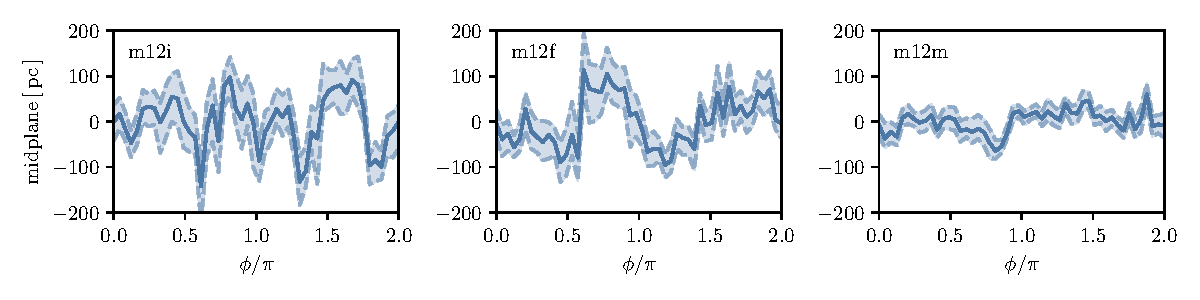
\includegraphics[width=7in]{fig/midplane_fit.pdf}
\end{center}
\caption{The local midplane determined at the fiducial Solar radius
($8.2\,\kpc$) for the three FIRE galaxies \mi{}, \mf{}, and \mm{} ({\em left},
{\em center}, and {\em right} panels). The local midplane is determined at a
position $\phi$ by taking the median height of all stars within $R=0.5\,\kpc$
and $z=1\,\kpc$ (in cylindrical coordinates). The procedure is performed again
using the new height $10$ times to converge on the local midplane height. In
order to allow for the possibility that the fiducial galactocentric coordinate
system is incorrect, we subtract the best fit $A\sin{(\phi+B)}+C$ curve from
each panel --- this figure is reproduced with the original midplane
determination (i.e. before subtracting the best fit sine curve) in
Appendix~\ref{app:lsr}. We then bootstrap resample $1000$ times on all stars
within a $2\,\kpc$ height of the fiducial midplane to determine $1\,\sigma
$ error bars, which we report as dashed lines.}
\label{fig:midplane}
\end{figure*}

\begin{figure*}
\begin{center}
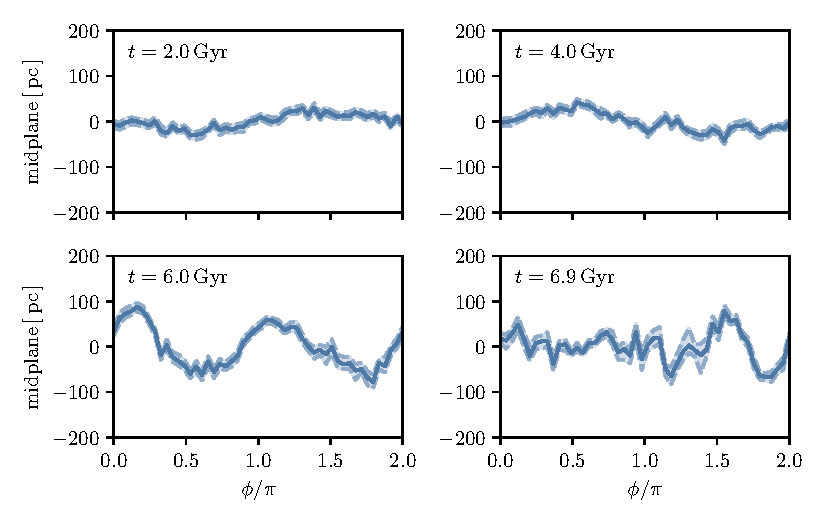
\includegraphics[width=5.5in]{fig/midplane_fit_chervinsim.pdf}
\end{center}
\caption{The local midplane determined at the fiducial Solar radius
($8.2\,\kpc$) for 4 different time steps from previously run toy simulations
of a Sagittarius encounter with the Milky Way \citep{2018MNRAS.481..286L}. As
before, we have subtracted the best fit $A\sin{(\phi+B)}+C$ curve to account
for inaccuracies in the galactocentric coordinate system. Error bars are
calculated as in Figure~\ref{fig:midplane}. (\Gus{Guessing here, need to
figure out what the panels actually show:}) The left two panels show the
midplane as a function of azimuth before the first encounter. As later
encounters occur, we can see that stronger midplane variations result. In
fact, one can see that an $m=2$ mode is excited in the third panel --- this is
consistent with Figure~17 of \citet{2018MNRAS.481..286L}, which shows that an
$m=2$ mode is excited (note that $m=0$ and $m=1$ modes are stronger, but these
are removed in our sine-curve subtraction).}
\label{fig:midplane_chervin}
\end{figure*}

\subsection{Velocity Variations} \label{ssec:lsr_var}
We also expect that the local standard of rest (LSR) should vary as a function
of azimuth. We perform this calculation in Appendix~\ref{app:lsr} to estimate
the components of the LSR as a function of azimuth, but performing a best-fit
subtraction to correct for misalignment of the original coordinate system (as
in the previous section) is more involved. Since we find that the variation in
the LSR is less pronounced than for the midplane, and since the dominant
effect is limited to $J_R$ (Figure~\ref{fig:many_orbit_wrong_ref}), we defer
this calculation to future work.

An interesting, qualitative calculation can be made based on the velocity
variations seen in e.g. \citet{2019arXiv190209569F}. The velocity variations
in this work (admittedly found with respect to $J_{\phi}$ or radius) are
$\sim5\text{--}10\,\kms$. The vertical frequency of the thin-disk and
thick-disk orbits are $\sim 0.09\,1/\Myr$ and $\sim0.06\,1/\Myr$,
respectively. By dimensional analysis, we therefore expect the midplane
offsets to be of order $\sim 57\text{--}170\,\pc$. We stress that this is a
rough calculation, but it shows that already we see evidence in the data from
velocities for midplane offsets on the order of what we see in both sets of
simulations.

\section{Discussion} \label{sec:discussion}
We have used high-resolution cosmological simulations to illustrate that we
expect the ``local midplane'' defined by stellar density to vary with azimuth
by up to $\pm 100$ pc, as a natural consequence of the non-axisymmetry of the
Galactic disk at small scales. While this is not in itself surprising or new,
we also demonstrate that extending the coordinate system established by our
local midplane to a global axisymmetric coordinate system spanning the
entirety of the Galactic disk introduces systematic error in computations of
the actions under this symmetry assumption, when starting from the present-day
positions and velocities of stars as measured by, e.g., \emph{Gaia}. These
systematic errors are most important for stars on thin disk-like orbits, where
they can be large enough to yield actions representative of orbits in the
thick disk. This effect is entirely due to the extension of a local to a
global coordinate system, and is separate from real diffusion in stellar
integrals of motion caused by interactions with these same deviations from
axisymmetry, such as resonant perturbation by spiral arms or scattering from
molecular clouds.

This finding has many implications for the study of the dynamics of stars in
what is normally considered the regime of the epicyclic approximation:
quasi-harmonic oscillations around a circular ``guiding center orbit.'' Here
we consider a few of those implications, starting with an estimate of the
region around the Sun where we expect an extension of the local axisymmetric
coordinate system, and therefore the epicyclic approximation, to still be
valid. This region is also where it should be feasible to perform ``dynamical
tagging'' in the thin disk; that is, using the computed orbits or integrals of
motion of field stars to match them with known open clusters.

\subsection{The size of the solar neighborhood} \label{sssec:neighborhood}
Given a local coordinate system, the amplitude and characteristic length scale
of the density fluctuations in the Galactic disk will determine how far this
coordinate system can be extended before introducing relevant systematic
errors in the computation of actions for thin-disk stars. We consider a $10\%$
error to be a criterion for the region around the Sun where the analysis of
the action-space distribution of stars on quasi-circular orbits, and therefore
the epicyclic approximation, can be expected to be valid. This leads to a
somewhat dynamically motivated definition of the ``solar neighborhood.'' Since
the motivation may be different for defining the solar neighborhood in, e.g.,
studies of the chemical distribution of the Galaxy, we propose the phrase
``dynamical solar neighborhood.'' We also point out that our use of a $10\%$
error is arbitrary.

To illustrate this concept, we first compute the absolute range of midplane
values for a given $\Delta \phi$ segment of the midplane. With the observer's
azimuth set to zero, we consider a region extending from $-\Delta \phi/2$ to
$\Delta\phi/2$. To translate this angular scale into a physical scale, we also
compute the chord length $\lambda$ for the chord extending from the observer
to $\pm \Delta\phi/2$ (see Figure~\ref{fig:fig_to_explain}). We repeat this
for each of $50$ bins in azimuth. Each bin is plotted in
Figure~\ref{fig:range_deltaphi} as a gray line, with the mean value in solid
blue and the $1\,\sigma$ dispersion as the dashed blue lines. We choose to
only consider the Solar circle to make the point that the midplane variation
as a function of azimuth (and not just Galactic radius) is important. However,
we note that because we use the range of midplane values, including regions of
each galaxy outside the Solar circle can only act to increase this range, and
therefore reduce the size of the dynamical solar neighborhood.

\begin{figure*}
\plotone{fig/fig_to_explain.pdf}
\caption{A cartoon explanation of Figure~\ref{fig:range_deltaphi}. An observer
is placed at the blue x in the plane of a backgrround galaxy (lime). For a
given $\Delta \phi$ (blue) centered on the observer, we record the range of
midplane values for this section of the Solar circle (orange). We plot the
value of the range against the value of $\Delta \phi$. We are also able to
convert the value of $\Delta \phi$ into a chord length (pink), which we plot
as a secondary, upper $x$-axis. We repeat the procedure for each initial
$\phi$ (gray lines), and also compute the mean and $\pm1\,\sigma$ values (dark
blue). We only consider the Solar circle to explore the impact of azimuthal
midplane variations, but similar effects are expected for radial midplane
variations.}
\label{fig:fig_to_explain}
\end{figure*}

\begin{figure*}
\begin{center}
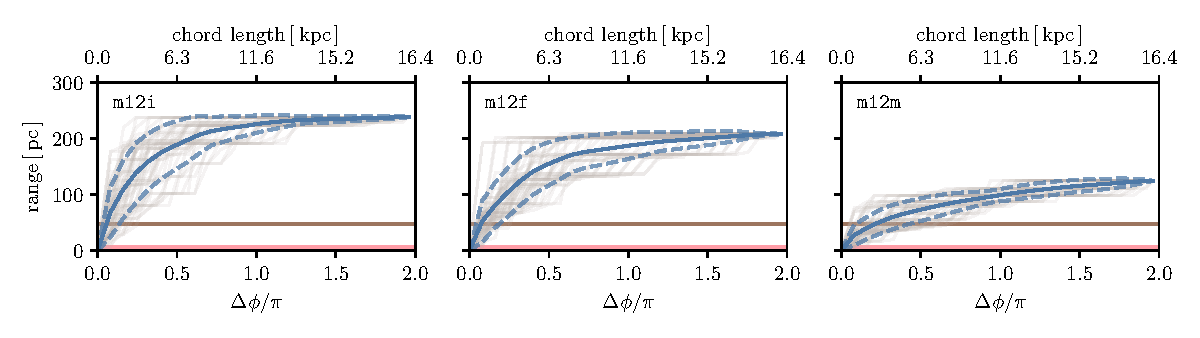
\includegraphics[width=6.8in]{fig/range_dphi.pdf}
\end{center}
\caption{The range of midplane heights encountered as a function of angular
width. At each angle $\phi$ from Figure~\ref{fig:midplane} we consider an
angular width of $\Delta \phi$ centered on $\phi$ and report the range of
midplane heights within that width. We repeat the procedure for each $\phi$
and plot the result as translucent gray lines. We also plot the mean range as
a solid blue line and the $\pm1\sigma$ lines as dashed blue lines. The upper
$x$-axis shows the chord length from the position $\phi$ to $\pm\Delta\phi/2$.
The horizontal \thincolor{} and \thickcolor{} lines shows the midplane
variation necessary to induce a $10\%$ error in $J_z$ for the thin-disk and
thick-disk orbits, respectively. A cartoon explanation of this Figure is given
in Figure~\ref{fig:fig_to_explain}. We only consider the Solar circle to
explore the impact of azimuthal midplane variations, but similar effects are
expected for radial midplane variations.}
\label{fig:range_deltaphi}
\end{figure*}

From Figure~\ref{fig:range_deltaphi} it is clear that the range of midplane
values spanned in a given $\Delta \phi$ quickly saturates at $\Delta \phi
\gtrsim \pi/2$ radians (i.e. one quarter of the way around the Galactic disk
from the Sun). At far smaller $\Delta \phi$ it reaches the level of deviation
required for a $10\%$ systematic error in $J_z$ for our fiducial
thin-disk-like orbit (\thincolor{} horizontal line in Figure
\ref{fig:range_deltaphi}). For the three simulations considered, the median
range exceeds this value at $\Delta \phi/\pi > 0.0073, 0.0096,
0.018\,\text{rad}$, with corresponding physical scales of $\lambda \sim 93.9,
123, 233\,\pc$ for \mi{}, \mf{}, and \mm{}, respectively. These can be
considered estimates of the range of validity for an extension of the locally
determined axisymmetric coordinate system, at least when it comes to the study
of stars on quasi-circular orbits.

The situation is more forgiving for the study of thick-disk-like orbits, where
a $10\%$ systematic error in $J_z$ requires a larger midplane
deviation (\thickcolor{} horizontal line in Figure~\ref{fig:range_deltaphi}).
In fact, the range of midplane variation in \mi{} just barely saturates to
cause such an error in $J_z$, with the midplane variation in \mf{} and \mm{}
never reaching such a value. For stars on halo-like orbits, extending the
local coordinate system globally is not likely to cause serious problems,
since the midplane deviations are relatively small compared to those needed to
produce $10\%$ systematic errors in the actions (\halocolor{}
horizontal line in Figure \ref{fig:range_deltaphi}). However, we caution that
the tendency of these midplane deviations is to \emph{inflate} the value of
$J_z$ whenever the midplane deviation is $\gtrsim z_{\text{max}}$, scattering
them into the region of action space normally associated with different
stellar populations and possibly contributing to confusion there (see
Figure~\ref{fig:Jz_hist} and discussion therein). This inflation is extremely
non-Gaussian (as the induced error is for all orbits, e.g.
Figure~\ref{fig:Jz_hist}), and is particularly troubling for the case of thin
disk stars, where the necessary midplane deviation is
$\sim5\textup{--}10\,\pc$.

\subsection{Consequences for disrupted cluster reconstruction}
\label{sssec:reconstruction}

We now consider the implications for attempts to reconstruct disrupting open
clusters by selecting ejected members based on their actions.

Suppose an open cluster of mass $m_c$ on an orbit with actions $\bm{J}_c$ is
disrupted. We would like to determine which stars with complete 6D phase-space
positions, for example in the {\em Gaia} dataset,\footnote{This is likely to
be more successful with DR3/4 than DR2, since upcoming data releases will
contain a far greater number of stars with radial velocities --- though
targeted, follow-up radial velocity surveys may allow this program to be
performed sooner.} are likely to be ejected members from that cluster. One
could generate an initial catalogue of candidate members by integrating the
cluster's orbit and selecting stars close to that orbit, accounting for the
fact that the stream of ejected stars will not exactly follow the orbit of the
cluster \citep[e.g.][]{2011MNRAS.413.1852E}.

One could then make a further selection by requiring that the action of each
field star $i$ be close to the cluster's actions to within some bound, i.e.
$\bm{J}_i \in V_e$, where $V_e$ is a volume centered on $\bm{J}_c$ and has size
comparable to the intrinsic action-space dispersion of the disrupting
cluster. This dispersion can be estimated as \citep[Section~8.3.3
of][]{2008gady.book.....B}
\beq \label{eq:action_disp}
\frac{\Delta J_i}{J_i} \sim \left(\frac{m_c}{M}\right)^{1/3}\text{,}
\eeq
where $m_c$ is the mass of the cluster and $M$ is the mass enclosed by the
cluster's orbit around the Galaxy, in this case assumed to be the mass inside
the Solar circle ($\sim 10^{11}\Msun$). Stars with actions within $V_e$ would
then be considered cluster members.

Two issues are immediately apparent with this approach. The first is that it
neglects the overall smooth distribution \emph{in action space} which will
contribute some stars to the selection by chance. For dissolving open clusters
in the thin disk, this background is likely to be significant, but we will
assume for the sake of argument that these foreground stars can be modeled
within the ``dynamical solar neighborhood'' where it is safe to extend the
local coordinate system. Since the effect of extending the coordinate frame
beyond this region is generally to inflate the actions computed for thin-disk
stars, using too large a volume is likely to under-estimate the density of the
smooth thin-disk-like component in action space, while scattering more
thin-disk stars onto thick-disk-like orbits and over-estimating the density of
the smooth thick-disk-like component.

The second issue, which is related to the point of this paper, is that based
on the results in our previous sections computing $\bm{J}_i$ for a field star
and directly comparing it to  $\bm{J}_c$ will have significant systematic
error if the cluster and field star are far enough apart to have significantly
different local midplanes (see Figure \ref{fig:range_deltaphi}). Since our
criterion for cluster membership (distance in action space) scales with the
cluster mass, the region where the search will succeed varies with cluster
mass as well. To illustrate this effect, we assume a cluster mass $m_c$ and
estimate the expected action-space dispersion from
Equation~\ref{eq:action_disp}. We then consult
Figure~\ref{fig:many_orbit_wrong_ref} to determine the midplane offset
necessary in order for the induced error in the vertical action to be the same
as the expected action-space dispersion. We perform this analysis for the
thin-disk-like and thick-disk-like orbits considered in
Section~\ref{ssec:quant}, assuming that the halo-like orbit is unlikely for
members of known open clusters (see Table~\ref{tab:real_clusters}). The result
for the allowable midplane offset for these two orbits in shown in
Figure~\ref{fig:cluster_offset} as a function of cluster mass.

With a characteristic midplane offset in hand, we use the relation in
Figure~\ref{fig:range_deltaphi}, which shows the typical midplane offset at
each $\Delta \phi$, to convert a given midplane offset into a typical
$\Delta\phi$. As in this Figure we assume the cluster is at the Solar circle
to obtain a physical scale, which we refer to as the ``neighborhood radius''
or $R_{\n}$. If the allowable midplane discrepancy is greater than the maximum
excursions recorded in the simulated galaxy, we simply report the maximum
chord length assuming an orbit on the Solar circle ($2\times8.2\,\kpc$). If an
observer is attempting to reconstruct a cluster with a given mass on a given
orbit, $R_{\n}$ gives the characteristic search distance between a field star
and the cluster within which an observer may not need to consider differences
in their respective local midplanes when computing actions. The result is
shown in Figure~\ref{fig:Rn_mc}. The solid lines indicate the neighborhood
values assuming the mean relation between midplane offset and $m_c$, and the
dashed lines show the $+1\,\sigma$ and $-1\,\sigma$ relations based on the 50
fiducial Solar positions in each simulation (as discussed in Figure
\ref{fig:range_deltaphi}). That this range is relatively wide illustrates the
strong $\phi$-dependence of the midplane offsets.

\begin{figure}
\plotone{fig/cluster_offset.pdf}
\caption{The $z$ offset necessary in order for the action error induced by our
midplane effect to be comparable to the intrinsic action dispersion from a
cluster of mass $m_c$. We compute the intrinsic dispersion from
Equation~\ref{eq:action_disp} and convert the dispersion to a $z$ offset using
the result from Figure~\ref{fig:many_orbit_wrong_ref}. We consider the result
for the thin and thick orbit (Table~\ref{tab:orbits}). Nearby open clusters
(Table~\ref{tab:real_clusters}) have orbits closest to the thin orbit.}
\label{fig:cluster_offset}
\end{figure}

Figure~\ref{fig:Rn_mc} shows that azimuthal midplane fluctuations will limit
the volume over which actions can be used to match stars to open clusters on
thin-disk-like orbits (\thincolor), depending on their mass. For
thick-disk-like orbits (\thickcolor), the tolerances are much more forgiving:
stars' actions can be compared over the entire Solar circle for nearly all
cluster masses, except at the very low-mass end in \mi . The neighborhood
around $\sim100\Msun$ clusters can be as small as $\sim x\,\pc$ but up to
$\sim y\,\kpc$ for \mi{} and \mf{}, though the situation is marginally better
for \mm{} with values ranging from $\sim a\,\kpc$ to $\sim b\,\kpc$. The
neighborhood values steadily increase with $m_c$, topping out at $\sim c\,\kpc$
for $\sim10^4\,\Msun$ clusters in
\mi{} and \mf{}. In \mm{}, the neighborhood size reaches the maximum allowed of
$16.4\,\kpc$ for clusters of mass $\sim m\,\Msun$. This figure also
underlines that the degree to which such an analysis will succeed depends
crucially on the expected degree of midplane fluctuations in the real Galaxy.
If the Milky Way is more like \mi , the range of action-space analysis
techniques like this is far more limited than if it more closely resembles
\mm{}.

We also compute $R_{\n}$ for each of the orbits of the real open clusters in
Table~\ref{tab:real_clusters}, using the midplane variations from
\mi{} as a conservative choice, since it has the largest degree of
midplane variation (Figure~\ref{fig:midplane}). We report the neighborhood
values for the mass of each cluster in the neighborhood column of
Table~\ref{tab:real_clusters}. Except for alphaPer, we find that the
neighborhood around each cluster is typically $\gtrsim x\,\pc$. This analysis
assumes that the MW resembles \mi{}, which is not necessarily true. However,
this step of our analysis is meant to be more illustrative than quantitative:
this calculation should actually be performed using real measurements of
variations in the MW's stellar midplane. Such measurements should be possible
in the near future with {\em Gaia}, with quality distance estimates the
crucial limiting factor, along with careful selction function modelling.

\begin{figure*}
\plotone{fig/Rn_vs_mc.pdf}
\caption{The dynamical neighborhood (discussed in
Section~\ref{sssec:neighborhood}) around an open cluster of mass $m_c$ for the
thin-disk, and thick-disk orbits (\thincolor{} and \thickcolor{},
respectively; see Table~\ref{tab:orbits}) and for each of the FIRE galaxies
considered here ---
\mi{}, \mf{}, and \mm{} ({\em left}, {\em center}, and {\em right} panels,
respectively). Given the $z$ offset for a cluster of mass $m_c$ computed in
Figure~\ref{fig:cluster_offset}, we convert this to a chord length using the
result from Figure~\ref{fig:range_deltaphi}. We interpret this chord length as
the ``neighborhood'' around the cluster, i.e. the distance from the cluster
one could go before the $J_z$ error induced by our midplane effect is
comparable to the intrinsic action dispersion of the cluster. When the $z$
offset is larger than the maximum range in Figure~\ref{fig:range_deltaphi}, we
report the maximum chord length ($2\times8.2\,\kpc$). We aso report the same
procedure but using the $\pm1\sigma$ lines from
Figure~\ref{fig:range_deltaphi}, which we plot here as dashed lines. For the
thick orbit (\thickcolor), the neighborhood is quite large and thus the effect
is negligible. However, for the thin orbit (\thincolor), which is closest to
the orbits of nearby open clusters (see Table~\ref{tab:real_clusters}), the
neighborhood is only a few hundred $\pc$ for low-mass clusters.}
\label{fig:Rn_mc}
\end{figure*}

\section{Conclusions}\label{sec:conclusion}
Actions have promise as excellent orbit labels. If the Galaxy can be
approximated as axisymmetric and 6D phase space positions can be measured
accurately and precisely enough, then the computed actions are invariant with
orbital phase. However, we have shown that the fact that the Galactic midplane
is not constant across the disk presents a significant complication to
computed actions actually being invariant. Our main conclusions are as
follows:

\begin{itemize}
\item We demonstrated that an inaccuracy in the Galactocentric coordinate
system induces time evolution in the {\em observed} actions
(Figures~\ref{fig:cartoon}\&\ref{fig:one_orbit_wrong_ref}). 

\item We interpret this time evolution as an error in the computed action
(Figure~\ref{fig:many_orbit_wrong_ref}). We focused on the effect that an
inaccuracy in the midplane has on the vertical action $J_z$. We found that in
order for there to be a $10\%$ error in $J_z$ (as defined by one half the middle
$90\uth$ percentile) one needs a midplane error of $\sim6\,\pc$ and
$\sim50\,\pc$ for a typical thin and thick disk orbit, respectively. The
fractional error is significantly less for halo orbits.

\item We pointed out that the error distribution of the actions induced by a
coordinate system error is very non-Gaussian. The distribution is bimodal with
{\em neither of the modes peaking at 
     null}. 
As a result, error
propagation is 
     complex
when considering actions.

\item We proposed that dynamical modelling across large regions of the disk is
susceptible to this type of error, since the assumption that our local
Galactic midplane is the global Galactic midplane is not true {\em a priori}.

\item To demonstrate the previous point, we measured the local Galactic
midplane along the Solar circle in three different high-resolution, zoom-in
simulations of Milky Way mass galaxies from the FIRE collaboration. We found
that the midplane varies by $\sim185, 162, 84\,\pc$ (middle $90\%$) for the
three galaxies we considered (\mi{}, \mf{}, and \mm{}, respectively).

\item This work emphasizes the importance of combining chemistry and dynamics.
Chemical tagging \citep{2002ARA&A..40..487F} and dynamical tagging must
complement and confirm each other. This was also recently pointed out by
\Gus{someone}.

\end{itemize}

While in this work we have focused on errors in action computation, all of our
conclusions also extend to studies of stars that simply rely on orbit
integration, since the computation of actions and orbit integrations are
essentially equivalent.

{\bf Add sentences about distribution function modeling}

Our main point is that the local midplane varies between different points in
the Galaxy. We do
not propose here what a modeler should use for the ``true'' global midplane,
since it depends on the particular problem being studied. Even without a
high-precision definition of the global Galactic midplane, current
observations from {\em Gaia} should soon permit a measurement of the real
azimuthal dependence of the midplane location.

\acknowledgments
We would like to thank Megan Bedell, Tobias Buck, and Todd Phillips
A.B. would like to thank Todd Phillips
for helpful discussions. A.B. was supported in part by the Roy \& Diana
Vagelos Program in the Molecular Life Sciences and the Roy \& Diana Vagelos
Challenge Award. 
%mm The work of \Gus{everyone} is supported by the Simons
%Foundation. \Gus{remove last sentence if everyone CCA affiliated}
M.-M.M.L. was partly supported by NSF grant AST18-15461.

\appendix
\section{Orbits} \label{app:orbits}
We plot the three orbits considered throughout the work
(Table~\ref{tab:orbits}) in Figure~\ref{fig:plot_orbits}.

\begin{figure*}
\plotone{fig/orbits.pdf}
\caption{The three orbits presented in Table~\ref{tab:orbits} and considered
throughout the work. We plot the thin, thick, and halo orbits in the {\em
left}, {\em center}, and {\em right} columns, respectively. The {\em upper}
row shows a plot of $x$ vs. $y$ while the {\em lower} row shows $R$ vs. $z$.}
\label{fig:plot_orbits}
\end{figure*}

\section{LSR Variations} \label{app:lsr}
We consider the variations of the LSR as a function of azimuth at the fiducial
solar circle ($R_{\odot} = 8.2\,\kpc$). At each azimuth, $\phi$, we take the
median velocity in cylindrical coordinates of all stars within $200\,\pc$ of
the position, following \citet{2018arXiv180610564S}. No best-fit subtraction
was performed as in Figure~\ref{fig:midplane}.

\begin{figure*}
\plotone{fig/lsr.pdf}
\caption{The local standard of rest (LSR) as a function of azimuth at the
fiducial Solar circle ($R_{\odot} = 8.2\,\kpc$). No best-fit subtraction is
performed here as we did in the case of the midplane
(Section~\ref{ssec:local_midplane}).}
\end{figure*}

\bibliography{references}

\end{document}
